%==================================Department Vision and Mission.tex================================

\newenvironment{Department Vision and Mission}

	\newpage
  \begin{center}
		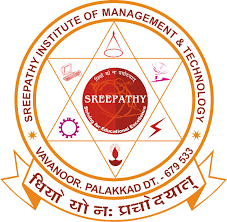
\includegraphics[scale=0.3]{figures/simatlogo.png}	
	\end{center}
	\begin{center}	

		%\vspace{1.5cm}
		\textbf{\large SREEPATHY INSTITUTE OF MANAGEMENT AND TECHNOLOGY, VAVANOOR\\}	
		\textbf{ \large KOOTTANAD 679533\\} 
            \vspace{0.8cm}
		\textbf{\large DEPARTMENT OF ARTIFICIAL INTELLIGENCE AND DATA SCIENCE\\}	
  
	\end{center}
	 \vspace{2cm}
	
	\begin{center}
		\textbf{\underline{\large Vision of Department}}
	\end{center}
 \begin{center}
	To empower future innovators in artificial intelligence and data science, through quality education, transformative research, and to harness it for a positive global impact leading to sustainable advancements in technology and society.
\end{center}
	
	\vspace{1cm}
	
	
	\begin{center}
		\textbf{\underline{\large Mission of Department}}
	\end{center}
 
	\begin{itemize}
  \item To build a skilled workforce for diverse career paths in industries ranging from healthcare and finance to cybersecurity and autonomous systems.
  \item To leverage research in AI and data science, to address critical societal challenges, drive economic growth, and improve the quality of life for individuals globally.
  \item To foster a culture of continuous learning and adaptation to stay abreast of rapid advancements in AI and data science through industry interaction.
\end{itemize}
	
	\thispagestyle{empty}
